\documentclass{project_report}
\usepackage[sfdefault]{libertine}
	\renewcommand*\familydefault{\sfdefault}
\usepackage{inconsolata}
\usepackage[T1]{fontenc}

\title{Website-Downloader \\and \\Search Engine}
\subject{Project - Network Programming}
\author{Kunal Pal, Thorsten Born}
\date{October 24, 2016}
\begin{document}
\maketitle

\section{Introduction} 

Throughout the network programming laboratory we have worked on coding tutorials involving different network protocols. The project offered during the session is to download a website in its entirety. However, this project also presents an opportunity to implement and test out ideas we have. In this project we have not only created a performant and efficient web-crawler but we have also used the data gathered to create a search engine. The primary goal of the crawler is to start from a given path and download the page pointed to by it. The crawler further processes the downloaded content looking for other links to follow and further download recursively.

In addition to extracting the links contained in a page, we also parse the page looking for tags and keywords. The links are also ranked using a simple reference-model. The keywords are further used to correlate with the search query provided by the user and serve search results that are most relevant to the given context.

From a technical perspective, this project also utilizes several other tools other than the c based socket api used throughout the lab sessions. E.g. it uses the mysql database driver to store and serve data in the backend. An extensive documentation is also generated using the doxygen library. The relevant configuration parameters are stored in an .ini file and passed as an argument in the command line. Several other technologies have also been used and will be discussed in detail in the following sections.

Section 2 elaborates on the algorithm used throughout this project while Section 3 details the extra features added. Finally Section 4 explains the specific involvements of the authors and concludes with a brief discussion on the applications and future scope of extending this project.

\section{Overview of the project}
This project, as the title suggests can be roughly divided into two separate but interdependent modules. The website downloader and the search engine. 
\subsection{Build System}
CMake has been used as the build system for this project. To keep the project modular and clean, the source code has been put into multiple header files to be included as needed. Additionally the several external libraries are also required to be linked for certain functionalities to work at all e.g. the mysql driver. This has grown the challenges of dependency management and linking exponentially and hence the use of CMake. 

CMake is an extension of the popular makefile based build system that is focused on making the build experience cross-platform. All the necessary libraries are included into the CMakelist.txt file which in turn generates a makefile with the proper locations of the libraries in the user's system. The makefile can be further compiled to produce the executables.

\subsection{Configuration parser}

The configurations for the projects are written in an .ini file and passed an an argument to the program. This utility makes the project more user friendly. Prominent parameters that are necessary for the program to work properly e.g. the save path, root url, hostname, port, mysql credentials are defined in the config file. The configurations can be changed at any instance and can be passed into the program without manually compiling the codes again.

An open-source library INIH has been used for this purpose. INIH helps parse the ini file and extract all the necessary variables using a handler defined in the code.

\subsection{Website Downloader}

The website downloader represents the client side of the networking in this project. The idea of a website downloader is simple - download the website from all the links contained in the website. The problem arises when we need to prepare the list of links by ourselves.

The program starts using a root url and fetches the contents of the remote path using proper GET http methods. The contents of this file, if html,  is then parser using a link extractor. In html, the href and src tags are used to define remote urls in the page. The link extractor looks specifically for these tags to identify the links. An open-source regex library SLRE has also been used to assist in the regular-expression matching in the link extractor.

The extracted links are then processed further to check if they point to the same source or to any external content. Since we are downloading the website, only the links that are local to the website are of interest in this purview. After the local links have been identified, they are url-encoded properly and then appended to the list of downloadable links. This stage of the program also categorizes the urls based on whether they point to an html page or any other resource such as image, css etc.

\begin{figure}[!hbt]
  \centering
  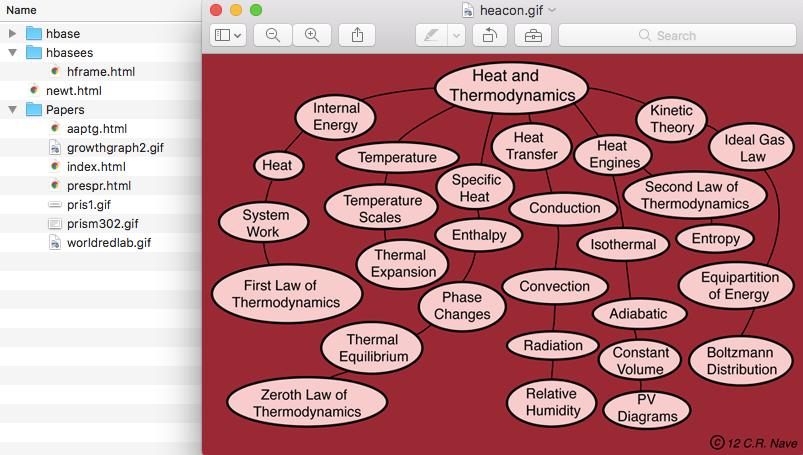
\includegraphics[width=0.8\textwidth]{downloader-sc}
  \caption{The folder structure of the downloaded website}
  \label{downloader-sc}
\end{figure}


In addition to extracting the url, the title and keywords are also compiled from the downloaded page. There informations help in the second part of the project, assisting in the search process of the search engine. Regular-expression matcher looks for any header tags that are present on the page and extracts their content to be later stored in the database.

Finally, the downloader saves the content of the fetched resource into a file. The directory structure specified in the url is preserved while saving the page. This helps in organizing the downloaded website as a replica of its' remote copy.

Fig. \ref{downloader-sc} illustrates the preservation of the directory structure. It also shows the capacity of the program to download binary image files.

\subsection{Search Engine}
The search engine uses the data fetched through the downloader to serve the user with relevant links. The search string is passed as a query in the GET path which is extracted using the regular expression matcher. The search string is then correlated with the keywords gathered by the website downloader. The results that match most are returned to the user as links to those pages.

Higher the correlation of a page with the search string, more likely it is to be returned on top of the search results. In addition to the correlation, the reference of the page is also taken into account. If a specific page is referred multiple times from other pages, that page is likely to be on top of the search results. It is needless to say that, if the query is empty, no results are returned.

Fig. \ref{search-sc} shows the results returned when the engine is searched using the word \emph{laws}. It is evident that the results are relevant to the user and ordered based on their association with the search string.

\begin{figure}[!hbt]
  \centering
  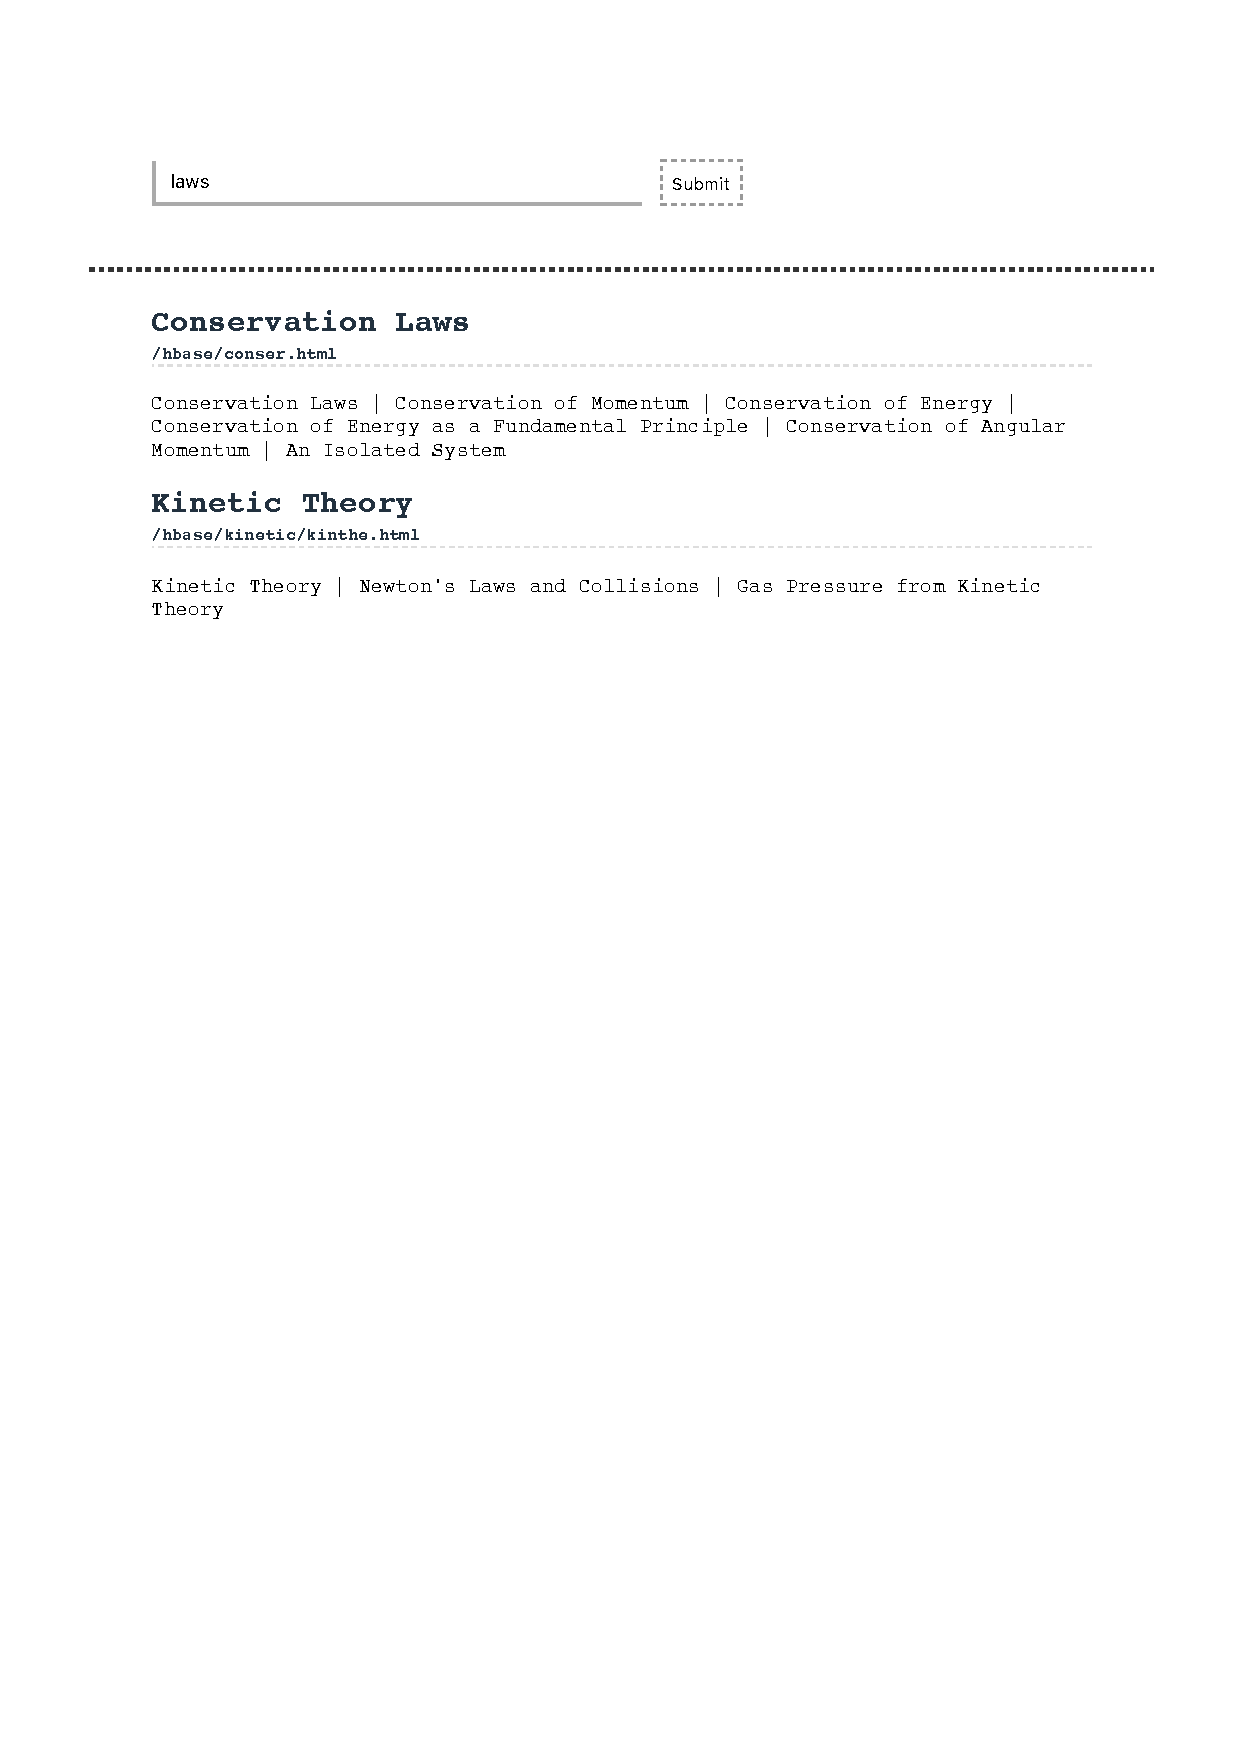
\includegraphics[trim={0 0 0 1.5cm},clip, width=\textwidth]{search-sc}
  \caption{The folder structure of the downloaded website}
  \label{search-sc}
\end{figure}

\section{Features}
The features added to the website downloader and the search engine are described in the following:
\begin{itemize}
	\item The website crawler takes all the configuration parameters from a config.ini file. Any variable information can be passed on to the program without compiling it again manually.
	\item Starting with the root path, the downloader resolves the url into its fundamental components, e.g. protocol, host, path etc. The ip of the url is resolved dynamically using the DNS lookup.
	\item The header of the fetch response is parsed to check the \emph{content type} tag. This helps determine if the page is or isn't a html page and in need of further link extraction.
	\item The downloader also parses the response code from the header. If the status code corresponds to a redirection, it further extracts the redirect location and fetches the page that it points to.
	\item The html content of the fetched document is parsed further in search of other links. The extracted links checked if local or external. Only the local links are followed further to be downloaded.
	\item The links extracted are url-encoded so that they can be looked up further.
	\item The url-encoded links along with the page title and the keywords are stored in a MySQL backend. This helps persist the data. If the program halts in the middle, the program can be restarted again from the same state instead of starting at the beginning.
	\item If the content type isn't \emph{text/html}, then the file is directly downloaded. The program can successfully download any kind of file - be it binary or text.
	\item \textbf{Doxygen documentation} is generated directly from the source codes. The comments, corresponding to each function includes the description of the function, input parameters and the return type. The documentation can be generated in either of \emph{html}, \emph{latex} and \emph{rtf}.
\end{itemize}

\section{Division of work}
The total work for this project has been separated between the two authors aforementioned. Author 1, Kunal Pal has handled data extraction, database management while the Author 2, Thorsten Born has developed the networking part of the project. The documentation, threading and the search engine part of the project has been developed by both the authors together.

\end{document}